%%%%%%%%%%%%%%%%%%%%%%%%%%%%%%%%%%%%%%%%%%%%%%%%%%%%%%%%%%%%%%%%%%%%%%%%%%
% File: Lecture_1.tex
% Authors: James Kress
% Date: February 1, 2014
% Description: 
%%%%%%%%%%%%%%%%%%%%%%%%%%%%%%%%%%%%%%%%%%%%%%%%%%%%%%%%%%%%%%%%%%%%%%%%%%

%<<<<<<<<<<<<<<<<<<<<<<<<<<<<<<<<<<<<<<<<<<<<<<<<<<<<<<<<<<<<<<<<<<<<<<<<<<<<<%
% Document package information
%>>>>>>>>>>>>>>>>>>>>>>>>>>>>>>>>>>>>>>>>>>>>>>>>>>>>>>>>>>>>>>>>>>>>>>>>>>>>>%
\documentclass[xcolor=dvipsnames]{beamer} 
%%%%%%%%%%%%%%%%%%%%%%%%%%%%%%%%%%%%%%%%%%%%%%%%%%%%%%%%%%%%%%%%%%%%%%%%%%
% File: _TeXdefs.tex
% Author: James Kress
% Date: January 25, 2014
% Description: A tex file containing the \usepackage declarations, and
%			   other document critial style settings.
%%%%%%%%%%%%%%%%%%%%%%%%%%%%%%%%%%%%%%%%%%%%%%%%%%%%%%%%%%%%%%%%%%%%%%%%%%

%-----------Package imports
\usepackage{graphicx}
\usepackage{pgfpages}
\usepackage{tikz}
\usepackage{latexsym}
\usepackage{verbatim}
%//////////END package imports


%----------Style elements
\useoutertheme{infolines} 
\usetheme{Frankfurt} 
\usepackage{../theme/beamercolorthemeoregon}
\setbeamertemplate{sections/subsections in toc}[default]
\setbeamertemplate{footline}
{
\leavevmode%
  \hbox{%
  \begin{beamercolorbox}[wd=.3\paperwidth,ht=2.25ex,dp=.75ex,center]{institute in head/foot}%
    \usebeamerfont{institute in head/foot}\insertshortinstitute
  \end{beamercolorbox}%
    \begin{beamercolorbox}[wd=.4\paperwidth,ht=2.25ex,dp=.75ex,center]{title in head/foot}%
      \usebeamerfont{title in head/foot}\insertshorttitle
    \end{beamercolorbox}%
  \begin{beamercolorbox}[wd=.3\paperwidth,ht=2.25ex,dp=.75ex,center]{date in head/foot}%
    \usebeamerfont{date in head/foot}\insertshortdate\hspace*{3em}
    \insertframenumber{} / \inserttotalframenumber\hspace*{1ex}
  \end{beamercolorbox}}%
  \vskip0pt%
}
%/////////END style elements


%---------Command Declarations
\DeclareGraphicsExtensions{.pdf, .jpeg, .png, .jpg}
\graphicspath{ {../images/} }
\newcommand{\className}{\text{CIS 410/510} \\ \text{Parallel Computing}}
\newcommand{\departmentName}{\textit{Department of Computer and 
									Information Science \\ University of Oregon}}
%/////////END command declarations


%---------Setup pdf properties
\hypersetup{
	pdfusetitle=true,
    bookmarks=true,         	% show bookmarks bar?
    unicode=false,          	% non-Latin characters in Acrobat’s bookmarks
    pdftoolbar=true,        	% show Acrobat’s toolbar?
    pdfmenubar=true,        	% show Acrobat’s menu?
    pdffitwindow=false,     	% window fit to page when opened
    pdfstartview={Fit},   		% fits the width of the page to the window    
    pdfauthor={},     % author
    pdfsubject={Parallel Programming},   	% subject of the document
    pdfcreator={},   			% creator of the document
    pdfproducer={}, 			% producer of the document
    pdfkeywords={University of Oregon, parallel programming}, 
    pdfnewwindow=true,      	% links in new window
    colorlinks=true,       		% false: boxed links; true: colored links
    linkcolor=white,          	% color of internal links
    hidelinks,
    citecolor=green,        	% color of links to bibliography
    filecolor=magenta,      	% color of file links
    urlcolor=cyan,           	% color of external links
    linktoc=page,
    pageanchor = true
}
%//////////END setup pdf properties


%END ALL


%<<<<<<<<<<<<<<<<<<<<<<<<<<<<<<<<<<<<<<<<<<<<<<<<<<<<<<<<<<<<<<<<<<<<<<<<<<<<<%
% END Document package information
%>>>>>>>>>>>>>>>>>>>>>>>>>>>>>>>>>>>>>>>>>>>>>>>>>>>>>>>>>>>>>>>>>>>>>>>>>>>>>%

%=============================================================================%
% Begining: Title Page Material
%=============================================================================%
\begin{document}
	\title[Collective Pattern]{Collective Pattern}
	\author[]{\className}
	\institute[\className]{\departmentName}
	\date{} 

	\titlegraphic{\centering 
		$\vcenter{\hbox{
\includegraphics[height=.31in,width=2.0in]{oregonLogo}}}$
	}

	\begin{frame}
		\maketitle
	\end{frame}
	
	\begin{frame}{Developer Training}
		\begin{center}
			
\includegraphics[width=0.4\textwidth]{images/OSNAP_logo} 
			
			Collective Pattern
			
			Information Security \& Cryptography
		\end{center}
	\end{frame}
	
	\begin{frame}{Cryptography on Intelligence}
		\begin{columns}
			\begin{column}{0.5\textwidth}
          Due to unforeseeable security leaks from the Allied Lunar Intelligence and Emergency Neutralization Squad, Central Intelligence has demanded that we tighten information security.
          \\~\\
          Executives of Central Intelligence have been given encryption keys. Together these keys can be used to encrypt and later decrypt data. They've requested that we design a system which requires all the keys to encrypt or decrypt data.
			\end{column}
			\begin{column}{0.5\textwidth}
				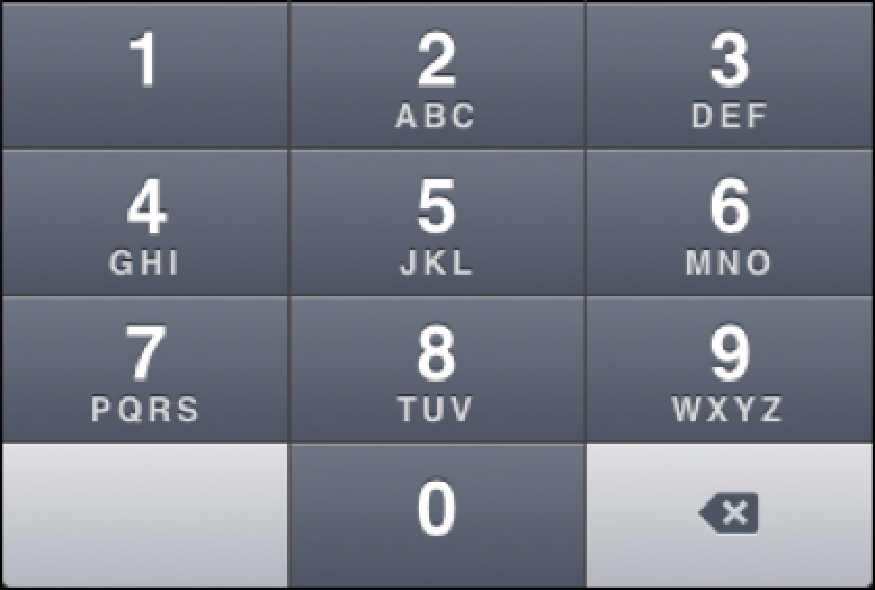
\includegraphics[width=\textwidth]{images/keypad}
			\end{column}
		\end{columns}
	\end{frame}
	
  \begin{frame}{Encryption Algorithm - Multi Key Xor}
		\begin{columns}
			\begin{column}{0.5\textwidth}
          XOR based encryption is a class of encryption algorithms in which the encryption
          and decryption keys are the same
					\\~\\
			    Each bit of the string is compared to the corresponding bit in a string of key
          bits for any number of keys. These keys will have different lengths,
          some combinations of key lengths lend themselves to trivial solutions. We will
          not make things that easy on the aliens. For messages longer than the length of
          our keys we will cycle back to the beginning of a key when we run out of key bits
      \end{column}
			\begin{column}{0.5\textwidth}
				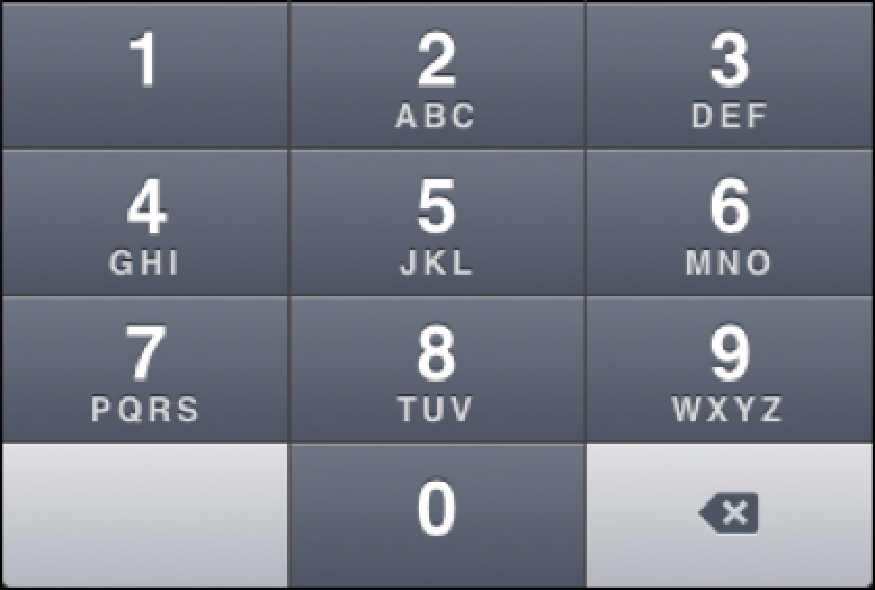
\includegraphics[width=\textwidth]{images/keypad}
			\end{column}
		\end{columns}
	\end{frame}
	
	\begin{frame}{Basic Solution}
		\begin{itemize}
			\item Provided: a file with intelligence to encrypt and decrypt
      \item Provided: a set of key files
			\item Required: Encrypt the file with the set of keys, print the ciphertext, decrypt the  ciphertext, print. If the first thing you printed isn't the same as the last, something is wrong.
			\item Template: \href{http://ix.cs.uoregon.edu/~dellswor/410}{\url{http://ix.cs.uoregon.edu/~dellswor/410}}
		\end{itemize}
	\end{frame}
	%--- Next Frame ---%
	
  \begin{frame}{Collective Reduce Operation}
		\begin{columns}
			\begin{column}{0.5\textwidth}
				\begin{itemize}
					\item N atomic data units, one output (a Gather Operation)
					\item Binary operation applied across inputs to produce the result
					\item Example: adding all input integers in a list to create output sum
          \item We will be xor'ing an input bit with a set of key bits to create output bit
				\end{itemize}
			\end{column}
			\begin{column}{0.5\textwidth}
				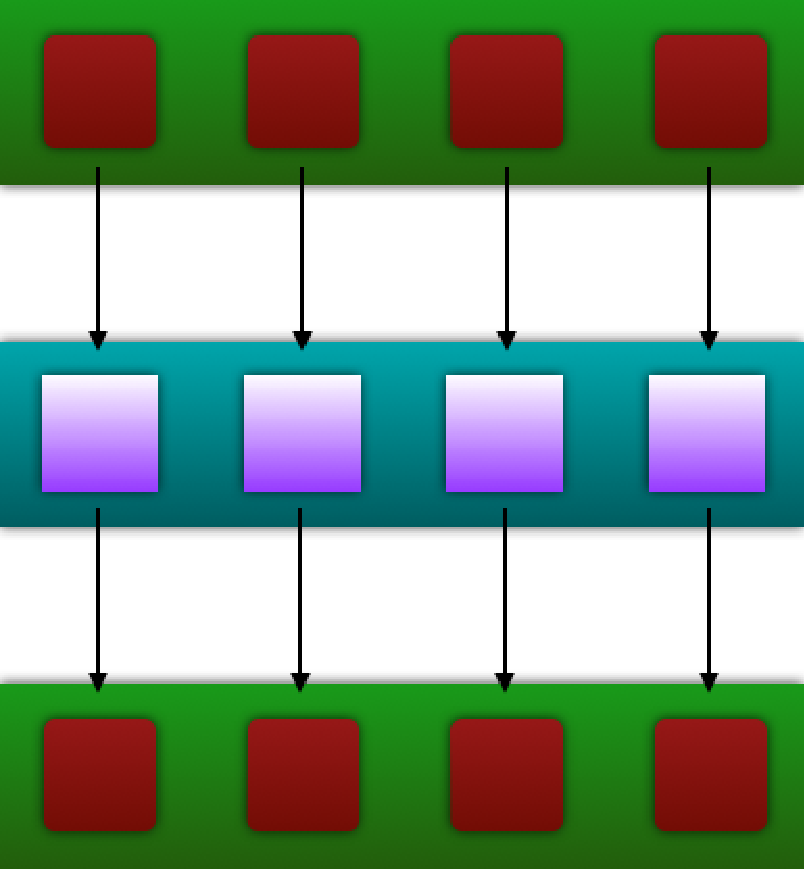
\includegraphics[width=\textwidth]{images/mapPattern}
			\end{column}
		\end{columns}
	\end{frame}
	
	
	\begin{frame}{Parallel Multiple Key Xor}
		\begin{itemize}
			\item Our solution is way too slow
			\item If only we had a team of developers to parallelize it...
      \item Use OpenMP, Cilk, TBB, or GPU assembly code, whichever seems appropriate.
		\end{itemize}
	\end{frame}
	
	\begin{frame}{Multiple Passwords - Example code}
		\begin{itemize}
      \item Example OpenMP code is stored on Mist
      \item Get into a directory you store source in 
			\item On Mist: run "cp -r /home/users/poliadz/OpenmpPasswordCracker ."
		\end{itemize}
	\end{frame}
  
  \begin{frame}{Key Points - Collective}
		\begin{itemize}
      \item Aggregate the results of applying an operation to a set of operands, producing a single output
      \item Design: Challenge in reduce is structuring the aggregation to expose maximum concurrency
			\item Identifying the correct parallelization is key to performance
		\end{itemize}
	\end{frame}
	
	%--- Next Frame ---%

\end{document}
%END ALL

